\documentclass[11pt,english]{article}

%%%%%%%%%%%%%%%%%%%%%%%%%%%%%%%%%%%%%%%%%%%%%%%%%%%%%%%%%%%
% Packages
%%%%%%%%%%%%%%%%%%%%%%%%%%%%%%%%%%%%%%%%%%%%%%%%%%%%%%%%%%%

% Package imports are stored in /assets/base-packages.tex
% Packages specific to this pset can be imported here.

\listfiles
% paper size & margins
\usepackage{fullpage}
\usepackage[showframe=false,margin=1in]{geometry}
\parindent=0pt

% font management
\usepackage{relsize}
\usepackage[T1]{fontenc} % for properly hyphenating words with accented chars
\usepackage[latin1]{inputenc}
\usepackage{babel}

% figure management
\usepackage{epsfig}
\usepackage{graphicx}
\usepackage{wrapfig}
\usepackage{subfig}
%\usepackage{subfigure}
\usepackage[belowskip=0pt,aboveskip=0pt,font=small]{caption}
%\usepackage{subcaption}
\setlength{\intextsep}{7pt plus 0pt minus 0pt}

% math
\usepackage{amsmath, amsthm, amssymb}
%\usepackage{amstext}
\usepackage{textcomp}
\usepackage{stmaryrd}
\usepackage{upgreek}
\usepackage{bm}
\usepackage{cases}
\usepackage{mathtools}

% assorted
\usepackage{url}
\usepackage{breakurl}
\usepackage[colorlinks=true]{hyperref}
\usepackage{xspace}
\usepackage{comment}
\usepackage{color}
\usepackage{afterpage}
\usepackage[normalem]{ulem}
\usepackage{enumitem}



%%%%%%%%%%%%%%%%%%%%%%%%%%%%%%%%%%%%%%%%%%%%%%%%%%%%%%%%%%%
% Shortcuts
%%%%%%%%%%%%%%%%%%%%%%%%%%%%%%%%%%%%%%%%%%%%%%%%%%%%%%%%%%%
\usepackage{assets/mysymbols}
%%% load AMS-Latex Package
\usepackage{amsmath,amsfonts}
\usepackage{amsthm,amssymb,amsopn}
\usepackage{bm} % bold symbol
\usepackage{bbm}

% define fonts
\newcommand{\vct}[1]{\boldsymbol{#1}} % vector
\newcommand{\mat}[1]{\boldsymbol{#1}} % matrix

%%%% Special math symbols
\newcommand{\field}[1]{\mathbb{#1}}
\newcommand{\R}{\field{R}} % real domain
\newcommand{\C}{\field{C}} % complex domain
\newcommand{\F}{\field{F}} % functional domain
%\newcommand{\T}{^{\top}\!\!} % transpose
\newcommand{\T}{^{\textrm T}} % transpose
\newcommand{\TN}{^{-\textrm T}} % transpose
\newcommand{\Lagr}{\mathcal{L}}


%%% define constant
\newcommand{\cst}[1]{\mathsf{#1}}

%% operator in linear algebra, functional analysis
\newcommand{\inner}[2]{#1\cdot #2}
%\newcommand{\norm}[1]{\|#1\|}
\newcommand{\twonorm}[1]{\|#1\|_2^2}
% operator in functios, maps such as M: domain1 --> domain 2
\newcommand{\Map}[1]{\mathcal{#1}}

% operator in probability: expectation, covariance,
\newcommand{\ProbOpr}[1]{\mathbb{#1}}
% independence
\newcommand\independent{\protect\mathpalette{\protect\independenT}{\perp}}
\def\independenT#1#2{\mathrel{\rlap{$#1#2$}\mkern2mu{#1#2}}}
% conditional independence
\newcommand{\cind}[3]{{#1} \independent{#2}\,|\,#3}
% conditional expectation
\newcommand{\cndexp}[2]{\ProbOpr{E}\,[ #1\,|\,#2\,]}

% operator in optimization
%\DeclareMathOperator{\argmax}{arg\,max}
%\DeclareMathOperator{\argmin}{arg\,min}
%\newcommand{\todo}[1]{{\color{red}#1}}


% environment
\newtheorem{thm}{Theorem}

\newcommand{\eat}[1]{}

\newcommand{\hide}[1]{}
%\newcommand{\solution}{{\Large \vspace{5mm} \textbf{{\color{red}Solution:}}\newline\newline}}

\newcommand{\diff}{\mathop{}\!\mathrm{d}}
\newcommand{\Vop}{\textrm{T}}
\newcommand{\norminf}[1]{\norm{#1}_\infty}

% definitions for PS4
\newcommand{\vecy}{\ensuremath{\mathbf{y}}\xspace}
\newcommand{\vecx}{\ensuremath{\mathbf{x}}\xspace}
\renewcommand{\argmax}{\operatornamewithlimits{argmax}}
\newcommand{\startsym}{\mbox{\scriptsize \texttt{<s>}}\xspace}
\newcommand{\stopsym}{\mbox{\scriptsize \texttt{</s>}}\xspace}
\newcommand{\best}{\ensuremath{\mathit{best}}\xspace}
\newcommand{\bestuptoi}{\ensuremath{\texttt{best}_{\leq i}}\xspace}
\newcommand{\bestuptot}{\ensuremath{\texttt{best}_{\leq t}}\xspace}
\newcommand{\completed}{\ensuremath{\texttt{comp}}\xspace}
\newcommand{\toptop}{\operatornamewithlimits{\mathbf{top}}}
\newcommand{\tuple}[1]{\ensuremath{\langle {#1} \rangle}}
\newcommand{\xuptot}{\ensuremath{\mathit{x}_{\leq t}}\xspace}


\renewcommand{\hide}[1]{}

%%%%%%%%%%%%%%%%%%%%%%%%%%%%%%%%%%%%%%%%%%%%%%%%%%%%%%%%%%%
% Title / Author
%%%%%%%%%%%%%%%%%%%%%%%%%%%%%%%%%%%%%%%%%%%%%%%%%%%%%%%%%%%
\begin{document}
\title{CS4803-7643: Deep Learning\\
Spring 2022 \\
Problem Set 4}

% NOTE: Any changes to instructor, TAs, or piazza link should be done in the file below
\author{Instructor: Zsolt Kira \\
TAs: Bhavika Devnani, Jordan Rodrigues, Mandy Xie, \\Yanzhe Zhang, Amogh Dabholkar, Ahmed Shaikh, \\ Ting-Yu Lan, Anshul Ahluwalia, Aditya Singh, Yash Jakhotiya\\
\\
Discussions: \url{https://piazza.com/gatech/spring2022/cs46447643a}}
\date{Due: Monday, April 4, 11:59pm}
\maketitle



\paragraph*{Instructions}
\begin{enumerate}
\item We will be using Gradescope to collect your assignments.  Please read the following instructions for submitting to Gradescope carefully!
     \begin{itemize}
          \item 
                For the \textbf{HW4 Writeup} component on Gradescope, please upload one single PDF containing the answers to all the theory questions, the report for the coding problems and the jupyter notebook \texttt{Machine\_Translation.ipynb} consisting of tests for parts of the code implementation. The solution to each problem/subproblem must be on a separate page. When submitting to Gradescope, please make sure to mark the page(s) corresponding to each problem/sub-problem.  
                Also, please make sure that your submission for the coding part only includes the files collected by the \texttt{collect\_submission} script, else the auto-grader will result in a zero, and we won't accept regrade requests for this scenario given the size of the class.
                Likewise, the pages of the report must also be marked to their corresponding subproblems. 

          \item
               For the coding problem, please use the provided \texttt{collect\_submission.py} script and
               upload the resulting file to the \textbf{HW4 Code} assignment on Gradescope. While we will
               not be explicitly grading your code, you are still required to submit it. Please make sure
               you have saved the most recent version of your code before running this
               script.

          \item
               Note: This is a large class and Gradescope's assignment segmentation features are essential.
               Failure to follow these instructions may result in parts of your assignment not being graded.
               We will not entertain regrading requests for failure to follow instructions.


               Please read \url{https://stats200.stanford.edu/gradescope_tips.pdf} for additional information on submitting to Gradescope.
     \end{itemize}

\item
    \LaTeX'd  solutions are strongly encouraged (solution template
     available on Canvas---Assignment 4 HW),
     but scanned handwritten copies are acceptable.
     Hard copies are \textbf{not} accepted.


\item We generally encourage you to collaborate with other students.

You may talk to a friend,
discuss the questions and potential directions for solving them. However, you need to write
your own solutions and code separately, and \emph{not} as a group activity.
Please list the students you collaborated with. \\ \\

\end{enumerate}


%%%%%%%%%%%%%%%%%%%%%%%%%%%%%%%%%%%%%%%%%%%%%%%%%%%%%%%%%%%
% Body
%%%%%%%%%%%%%%%%%%%%%%%%%%%%%%%%%%%%%%%%%%%%%%%%%%%%%%%%%%%

\section{Collaborators [0.5 points]}

Please list your collaborators and assign this list to the corresponding section of the outline on Gradescope. If you don't have any collaborators, please write 'None' and assign it to the corresponding section of the Gradescope submission regardless.


\section{Recurrent Neural Networks and Transformers}
\begin{enumerate}[start]

\item
\textbf{[Vanilla RNN for parity function: 3 points]}
Let us define a \emph{sequence parity function} as a function that takes in a sequence of binary inputs  
and returns a sequence indicating the number of 1's in the input so far; specifically, if at time $t$ 
the 1's in the input so far is odd it returns 1, and 0 if it is even. 
For example, given input sequence $[0, 1, 0, 1, 1, 0]$, 
the parity sequence is $[0, 1, 1, 0, 1, 1]$. 
Let $x_t$ denote the input at time $t$ and $y_t$ be the boolean output of this parity function at time $t$. 

Design a vanilla recurrent neural network to implement the parity function. 
Your implementation should include the equations of your hidden units and 
the details about activations with different input at $x_t$ (0 or 1). 

Hint: Recall that we have implemented AND and OR functions in HW3, which may be useful here. 

\item
\textbf{[LSTM for parity function: 5 points]}
Let us recall different gates in an LSTM Network. First gate is the "forget gate layer":\\
\begin{equation}
    f_t = \sigma (W_f.[h_{t-1}, x_t] + b_f)
\end{equation}
where $f_t$ is the output of forget gate, $W_f$ is the weight matrix, $h_{t-1}$ is the hidden state of step \textit{t-1}, $x_t$ is the current input and $b_t$ is the bias value. \\
Next we have "input gate layer":\\
\begin{equation}
    i_t = \sigma (W_i.[h_{t-1}, x_t] + b_i) \\
\end{equation}
\begin{equation}
    \Tilde{C_{t}} = \tanh (W_C.[h_{t-1}, x_t] + b_C) 
\end{equation} \\
where $i_t$ decides which values we will update and $\Tilde{C_{t}}$ are the new candidate values that could be added to the cell state. Next we have new cell state candidate values:
\begin{equation}
    C_t = f_t * C_{t-1} + i_t * \Tilde{C_{t}} 
    \label{eqn:xor}
\end{equation}
Finally, we have the output and hidden state
\begin{equation}
   o_t = \sigma (W_o .[h_{t-1}, x_t] + b_o) \\
\end{equation}
\begin{equation}
    h_t = o_t * \tanh(C_t)
\end{equation}

Design an LSTM Network for the bit parity problem mentioned in Question 1. Specifically, provide values for $W_f$, $b_f$, $W_i$, $b_i$, $W_C$, $b_C$, $W_o$ and $b_o$ such that the cell state $C_t$ stores the parity of bit string. Please mention any assumptions you make. For this problem, you can assume below for Sigmoid and $\tanh$ function: \\
\begin{equation}
    \sigma(x) = \begin{dcases}
    1,& \text{if } x > 0\\
    0,              & \text{otherwise}
\end{dcases}
\end{equation}
\begin{equation}
    \tanh(x) = \begin{dcases}
    1,& \text{if } x > 0\\
    0,              & x = 0\\
    -1,& \text{if } x < 0
\end{dcases}
\end{equation}


Hint: Recall that XOR of x and y can be represented as ($x\land \bar{y}$) $\lor$ ($\bar{x} \land y$). Think about how you can leverage this information for equation \eqref{eqn:xor}.

\item
\textbf{[When to Stop in Beam Search: 5 points]}
Beam Search is a widely-used technique for decoding the most likely sequence from sequence models. 
But it is difficult to decide when to stop beam search to obtain optimality because hypotheses can finish in different steps. 
In this question, we will develop a formal understanding of the stopping criteria in beam search. 

Let $\vec{x}$ denote the input upon which we condition our sequence model. Let $\vecy$ denote the output sequence. 
Let $\vecy_{<t}$ be a shorthand notation for the sub-sequence $(y_{0}, y_{1}, \ldots, y_{t-1})$. 
We say that a sequence (or hypothesis as they are sometimes referred to in this literature) 
\vecy is \emph{completed} ($\completed(\vecy) = true$), if its last token is \stopsym, \ie,
\[
\completed(\vecy) = true \leftrightarrow (\vecy_{|\vecy|} = \stopsym)
\]
in which case it will not be further expanded in beam search.

With this notation, we can write down the maximum a-posteriori inference problem as: 
\begin{align}
	\vecy* = \argmax_{\vecy} & \quad \prod_{t\leq |\vecy|}^{} p(y_t | \vecx,\vecy_{<i}) \\ 
	\st & \quad \completed(\vecy) = true
\end{align}

We use beam search to find the (approximate) best output $\vecy^*$
At time $t$, let $B_{t-1}$ denote the beams so far. Thus, $B_{t-1}$ is a $b$-length list consisting of $\tuple{\vecy, s}$ pairs, 
\ie, $B_{t-1} = \big( \, \tuple{\vecy^1, s^1}, \ldots, \tuple{\vecy^b, s^b} \, \big)$, where $\vecy^i$ is a $(t-1)$-length sequence (a beam) 
and $s^i$ is its associated score (sum of log-conditional probabilities), \ie $s^i =  \sum_{j=1}^{t-1} \log p(y^i_j \mid \vecx, \vecy^i_{<j}) $. 

Let $\circ$ denote a concatenation operation, \ie $\vecy \circ y_t$ represents a beam expansion where 
$\vecy$ is concatenated with $y_t$. 
Beam search can be then be formalized via a $\toptop^b$ operator that selects (quite literally) the top-$b$ scoring items 
in an expanded list of beams:  
\begin{align}
	B_t\! &= \!\toptop^b  
	\big\{\, \tuple{\vecy \circ y_t, \ s + \log p(y_t | \vecx, \vecy_{<t})} \mid \tuple{\vecy\!, s} \in B_{t-1} \, \big\}
\end{align}

Let $\bestuptot$ be the best completed hypothesis so far (up to step $t$), \ie
\begin{align}
    \bestuptot \quad \overset{\Delta}{\textbf{=}} \quad \max \Big\{ s \mid \tuple{\vecy,s} \in \cup_{j \leq t} B_t,  \completed(\vecy) = true \Big\}
\end{align}

Notice that if there no completed beam till time $t$, $\bestuptot$ is undefined/empty. 

Now, for the proof.

Assuming that $\bestuptot$ is defined at time $t$ and the current highest scoring beam in $B_t$ (\ie $\vecy^1$) scores worse than or equal to $\bestuptot$, \ie $s^1 \le \bestuptoi$, 
prove that there is no need to run beam search out further. That is, 
prove that the current best completed beam (corresponding to $\bestuptot$) is the overall highest-probability completed beam  
and future steps will be no better.

\item
\textbf{[Exploding Gradients: 5 points]}
Learning long-term dependencies in recurrent networks suffers from a particular numerical challenge -- 
gradients propagated over many time-steps tend to either `vanish' (i.e. converge to 0, frequently) or `explode' (\i.e. diverge to infinity; rarely, but with more damage to the optimization). To study this problem in a simple setting, consider the following recurrence relation without any nonlinear activation function or input $x$:

\begin{equation} \label{eq:simple_recurrence}
h_{t} = W^\top h_{t-1}
\end{equation}

where $W$ is a weight sharing matrix for recurrent relation at any time $t$. Let $\lambda_1, ..., \lambda_n$ be the eigenvalues of the weight matrix $W \in \C^{n \times n}$. Its spectral radius $\rho(W)$ is defined as: 

\begin{align}
\rho(W) = \text{max}\{|\lambda_1|, ... ,|\lambda_n| \}
\end{align}

Assuming the initial hidden state is $h_0$, write the relation between $h_t$ and $h_0$ and explain the role of the eigenvalues of $W$ in determining the `vanishing' or `exploding' property as $t\gg0$.

\item
\textbf{[Transformer as GNN: 5 points; Extra credit for both 4803 and 7643]}
Learning representations of inputs is the bedrock of all neural networks.

In recent years, Transformer models have been widely adapted to sequence modeling tasks in the vision and language domains, while Graph Neural Networks (GNNs) have been effective in constructing representations of nodes and edges in graph data. In the following questions we will explore both Transformers and GNNs, and draw some connections between them.

\textbf{Background:}

Let us first take a look at a graph model. We define a directed graph $G = \{V,E\}$ where $V$ is the set of all vertices and $E$ is the set of all edges. For $\forall v_i \in V$, let us define $\mathcal{N}(v_i)$ as the set of all of $v_i$'s neighbors with outgoing edges towards $v_i$. $v_i$ has a state representation $h_i^{t}$ at each time step $t$.

The values of $h_i^{t}$ are updated in parallel, using the same snapshot of the graph at a given time step. The procedures are as follows: We first need to aggregate the incoming data $H'_{it} = \{f_{ji}(h_j^{t})| \forall j, v_j \in \mathcal{N}(v_i)\}$ from neighbors using the function $Agg(H'_{it})$. Note that the incoming data from each neighbor is a transformed version of its representation using function $f_{ji}$. The aggregation function $Agg(H'_{it})$ can be something like the summation or the mean of elements in $H'_{it}$. 

Say the initial state at time step 0 is $h_i^{0}$. Now let us define the update rule for $h_i^{t}$ at time step $t+1$ as the following:
        \begin{equation} \label{eq:GNN}
            h_i^{t+1} = q(h_i^{t}, Agg(H'_{it}))
        \end{equation}
    where $q$ is a function - $Q_{t}: \{H_{t},Agg(H'_{t})\} \rightarrow H_{t}$, where $H_{t} = \{h_n^{t}| \forall n, v_n \in V\}$. 

Now, let us take a look at Transformer models. Recall that Transformer models build features for each word as a function of the features of all the other words with an attention mechanism over them, while RNNs update features in a sequential fashion. 

To represent a Transformer model's attention mechanism, let us define a feature representation $h_i$ for word $i$ in sentence $S$. We have the standard equation for the attention update at layer $l$ as a function of the each other word $j$ as follows:
\begin{align}
    h_{i}^{l+1} &= \texttt{Attention}(Q^{l}h^{l}_{i}, K^{l}h^{l}_{j}, V^{l}h^{l}_{j}) \label{eq: Attention1}\\
     &= \sum_{j\in S} \big( \texttt{softmax}_{j} (Q^{l}h^{l}_{i} \cdot K^{l}h^{l}_{j}) V^{l} h^{l}_{j} \big) \label{eq: Attention2}
\end{align}
where $Q^{l}, K^{l}, V^{l}$ are weight matrices for ``Query'', ``Key'', and ``Value''. $Q$ is a matrix that contains vector representations of one word in the sentence, while $K$ is a matrix containing representations for all the words in the sentence. $V$ is another matrix similar to $K$ that has representations for all words in the sentence. As a refresher for your knowledge about the Transformer model, you can refer to this \href{https://arxiv.org/abs/1706.03762}{paper}.


Based on the above background information, answer the following questions:

\begin{enumerate}
    \item 
    
    If the aggregation operation for $Agg(H'_{it})$ is the summation of representation of all adjacent vertices, rewrite the equation \ref{eq:GNN} by replacing $Agg(H'_{it}))$ in terms of $\mathcal{N}$, $f$, and $h$.
    
    \item Consider the directed graph G in Fig~\ref{fig: graph}.
    \begin{figure}[h] 
        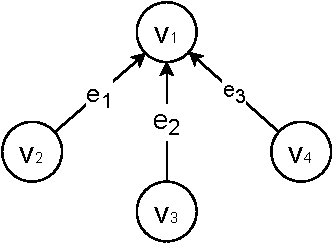
\includegraphics[scale = 0.8]{assets/graph.pdf}
        \centering
        \caption{}\label{fig: graph}
    \end{figure}
    The values for the vertices at time step t are as follows:
    \begin{equation}
        h_1^{t} = [1, -1] \quad h_2^{t} = [-1, 1] \quad h_3^{t} = [0, -1]\quad h_4^{t} = [1, 0]
    \end{equation}
    
    The aggregation function $Agg(H'_{1t})$ is:
    \begin{equation}
        Agg(H'_{1t}) = [0.6, 0.2, 0.2] \begin{bmatrix}
           f(h_{2}^{t}) \\
           f(h_{3}^{t}) \\
           f(h_{4}^{t})
         \end{bmatrix}
    \end{equation}
    
   And the function $f$ on all the edges is:
    \begin{equation}
        f(x) = 2x
    \end{equation}
    
    Now, given that
    \begin{equation}
        h_1^{t+1} = q(h_1^{t}, Agg(H'_{1t})) = W(h_1^{t})^{T} + max\{Agg(H'_{1t}),0\}
    \end{equation}where $W = [1,1]$, what is the updated value of $h_1^{t+1}$?
\end{enumerate}

\begin{enumerate}[resume]
    \item Consider the graph G in question (b). We want to alter it to represent the sentence "I eat red apples" (4 word tokens) as a fully connected graph. Each vertex represents one word token, and the edges represent the relationships among the tokens. How many edges in all would graph G contain? Notice that the edges are directed and a bi-directional edge counts as two edges.
    \item Using equations \ref{eq:GNN} and \ref{eq: Attention2}, show that the Transformer model's single-head attention mechanism is equivalent to a special case of a GNN. 
    \item An ongoing area of research in Transformer models for NLP is the challenge of learning very-long-term dependencies among entities in a sequence. Based on this connection with GNNs, why do you think this could be problematic? 
\end{enumerate}


\end{enumerate}

\section{Paper Review [Extra credit for 4803, regular credit for 7643]}

% Point values for paper review defined in the question file
For this homework's paper review section, we turn to the interesting and increasingly important field of Explainable AI. 

\vspace{2mm}

The following paper \textbf{Multimodal Explanations: Justifying Decisions and Pointing to the Evidence}, which was presented at CVPR 2018, introduces a unique multi-modal approach to explainability by joint textual rationale generation and attention visualization - in the tasks of visual question answering (VQA) and activity recognition. This was a major improvement over pre-existing unimodal explainability techniques (such as the ones covered in the coding section of HW3), with the results showing complementary explanatory strengths from the visual and textual explanations. 

\vspace{2mm}

The paper can be viewed \href{https://openaccess.thecvf.com/content_cvpr_2018/html/Park_Multimodal_Explanations_Justifying_CVPR_2018_paper.html}{here}.
\vspace{2mm}
The evaluation rubric for this section is as follows:
\begin{enumerate}[resume]
\item
\textbf{[2 points]}
Briefly summarize the key contributions, strengths and weaknesses of this paper.

\item
\textbf{[2 points]}
What is your personal takeaway from this paper? This could be expressed either in terms of relating the approaches adopted in this paper to your traditional understanding of explainability techniques, or potential future directions of research in the area which the authors haven't addressed, or anything else that struck you as being noteworthy. 

\end{enumerate}

Guidelines: Please restrict your reviews to at least one paragraph per question, but no more than 350 words (total length for answers to both of the above questions). Please write separate answers for each question to assist in Gradescope grading.

\section{Coding: Machine Translation with Seq2Seq and Transformers}

\textbf{[20 points]}
The coding part of this assignment will consist of implementation of sequence models and a Transformer model for Engish-German translation. 
To get started, download the code zip file from \href{https://www.cc.gatech.edu/classes/AY2022/cs7643_fall/assets/assignment4.zip}{here}. Also, be sure to append the completed report (PPT template available in the zip folder) \emph{and} the Jupyter notebook \texttt{Machine\_Translation.ipynb} (as mentioned in the instructions) 
to the PS4 theory solutions and upload them as one PDF on Gradescope under HW4 writeup. \\


Points breakdown:
\begin{itemize}
    \item HW4 Code
    \begin{itemize}
        \item Autograder [11 points]
    \end{itemize}
    \item HW4 Writeup
    \begin{itemize}
        \item Theory Answers [18 points for 4803/ 22 points for 7643]
        \item Report PDF [9 points]
        \begin{itemize}
            \item Description and results for Seq2Seq [4 points]
            \item Description and results for Transformer [5 points]
        \end{itemize}
        \item Jupyter Notebook as PDF
    \end{itemize}
\end{itemize}

\end{document}
